\documentclass[a4paper]{article}

% Packages
\usepackage[utf8]{inputenc}
\usepackage{biblatex}
\usepackage[english]{babel}
\usepackage{amsmath, amssymb}
\usepackage{graphicx}
\usepackage{hyperref}
\usepackage{geometry}
\usepackage{amsmath}
\usepackage{bm}
\geometry{a4paper, total={5.6in,9in}}
\addbibresource{bibl.bib}

% Title and Author
\title{SLAM performance predicition}
\author{Mauro Tellaroli \\ 
    \small Statistical Methods for Maching Learning \\ 
    \small Università degli Studi di Milano
}
\date{}

\begin{document}

\maketitle

\begin{center}
\begin{minipage}{0.9\textwidth}\textit{
I declare that this material, which I now submit for assessment, is entirely my own work and has 
not been taken from the work of others, save and to the extent that such work has been cited and 
acknowledged within the text of my work. I understand that plagiarism, collusion, and copying 
are grave and serious offences in the university and accept the penalties that would be imposed should 
I engage in plagiarism, collusion or copying. This assignment, or any part of it, has not been previously 
submitted by me or any other person for assessment on this or any other course of study.}
\end{minipage}
\end{center}
\vspace{2em}

\section{Introduction}
In the field of autonomous mobile robot, the Simultaneous Localization And Mapping (SLAM) represents
one of the most significant problems. As the name suggests, the goal of the SLAM is incrementally obtain 
from a mobile robot a map of the environment and simultaneously locate the robot's position inside it.
The difficulty of the SLAM problem is that to precisely localize itself, the robot needs an accurate map,
while to obtain an accurate map, it needs an accurate localization inside the map. This type of problems is 
called chicken-and-egg problem.

\subsection{SLAM methods}
In the last 30 years several approaches have been developed to solve the SLAM problem leading to methods 
extensively used in both common and industrial scenarios. The main paradigms \cite{Stachniss2016} used are:
\begin{itemize}
    \item Extended Kalman Filter: a vector containing the estimates of the robot position and the environment 
    landmark is used. In addition, a matrix composed of the correlations between the positions and landmark
    estimates is also used. Both the vector and the matrix are updated using the extended Kalman Filter.
    \item Particle Filter: the Monte Carlo method is used to sample the possible states of the robot. A
    random sample is called a particle and it's composed of the robot position and a map estimate. The main 
    steps are: predict the robot’s pose for each particle, update particle weights based on sensor data,
    resample particles according to their weights, and update each particle’s map.
    \item Graph-based: a graph is used where nodes represent robot poses or landmarks, and edges represent
    spatial constraints derived from sensor observations or odometry. The SLAM problem is formulated as a 
    graph optimization task, where the goal is to find the configuration of nodes that best satisfies all 
    constraints, typically using nonlinear optimization techniques.
\end{itemize}

\subsection{Accuracy of SLAM methods}
The heterogeneity of SLAM methods makes it difficult to find a measure that can evaluate their godness.
Many approaches rely on manual evaluation or utilize information derived from the specific algorithm.
Nowadays the most used metric is the Absolute Pose Error (APE)\cite{APE}. The APE measures the difference between 
the estimated trajectory produced by the SLAM algorithm and the ground truth trajectory, focusing on the global 
consistency of the estimated poses. The big advantage of the APE is that it allows for a quantitative assessment 
of how well the SLAM algorithm reconstructs the robot's trajectory over time, independent of the internal workings 
of the specific method used.

The APE is composed of two sub-metrics:
\begin{enumerate}
    \item The Absolute Translational Error (ATE): it measures the difference in position, typically using the 
    Euclidean distance between corresponding poses.
    \item The Absolute Rotational Error (ARE): it measures the difference in orientation, often computed as the 
    angular distance between corresponding rotations.
\end{enumerate}
Figure \ref{fig:APE} and \ref{fig:trajectories} show respectively the ATE variation over time and the difference
between the ground truth and the robot estimated trajectory during an environment exploration.

\begin{figure}[htbp]
    \centering
    \begin{minipage}{0.48\textwidth}
        \centering
        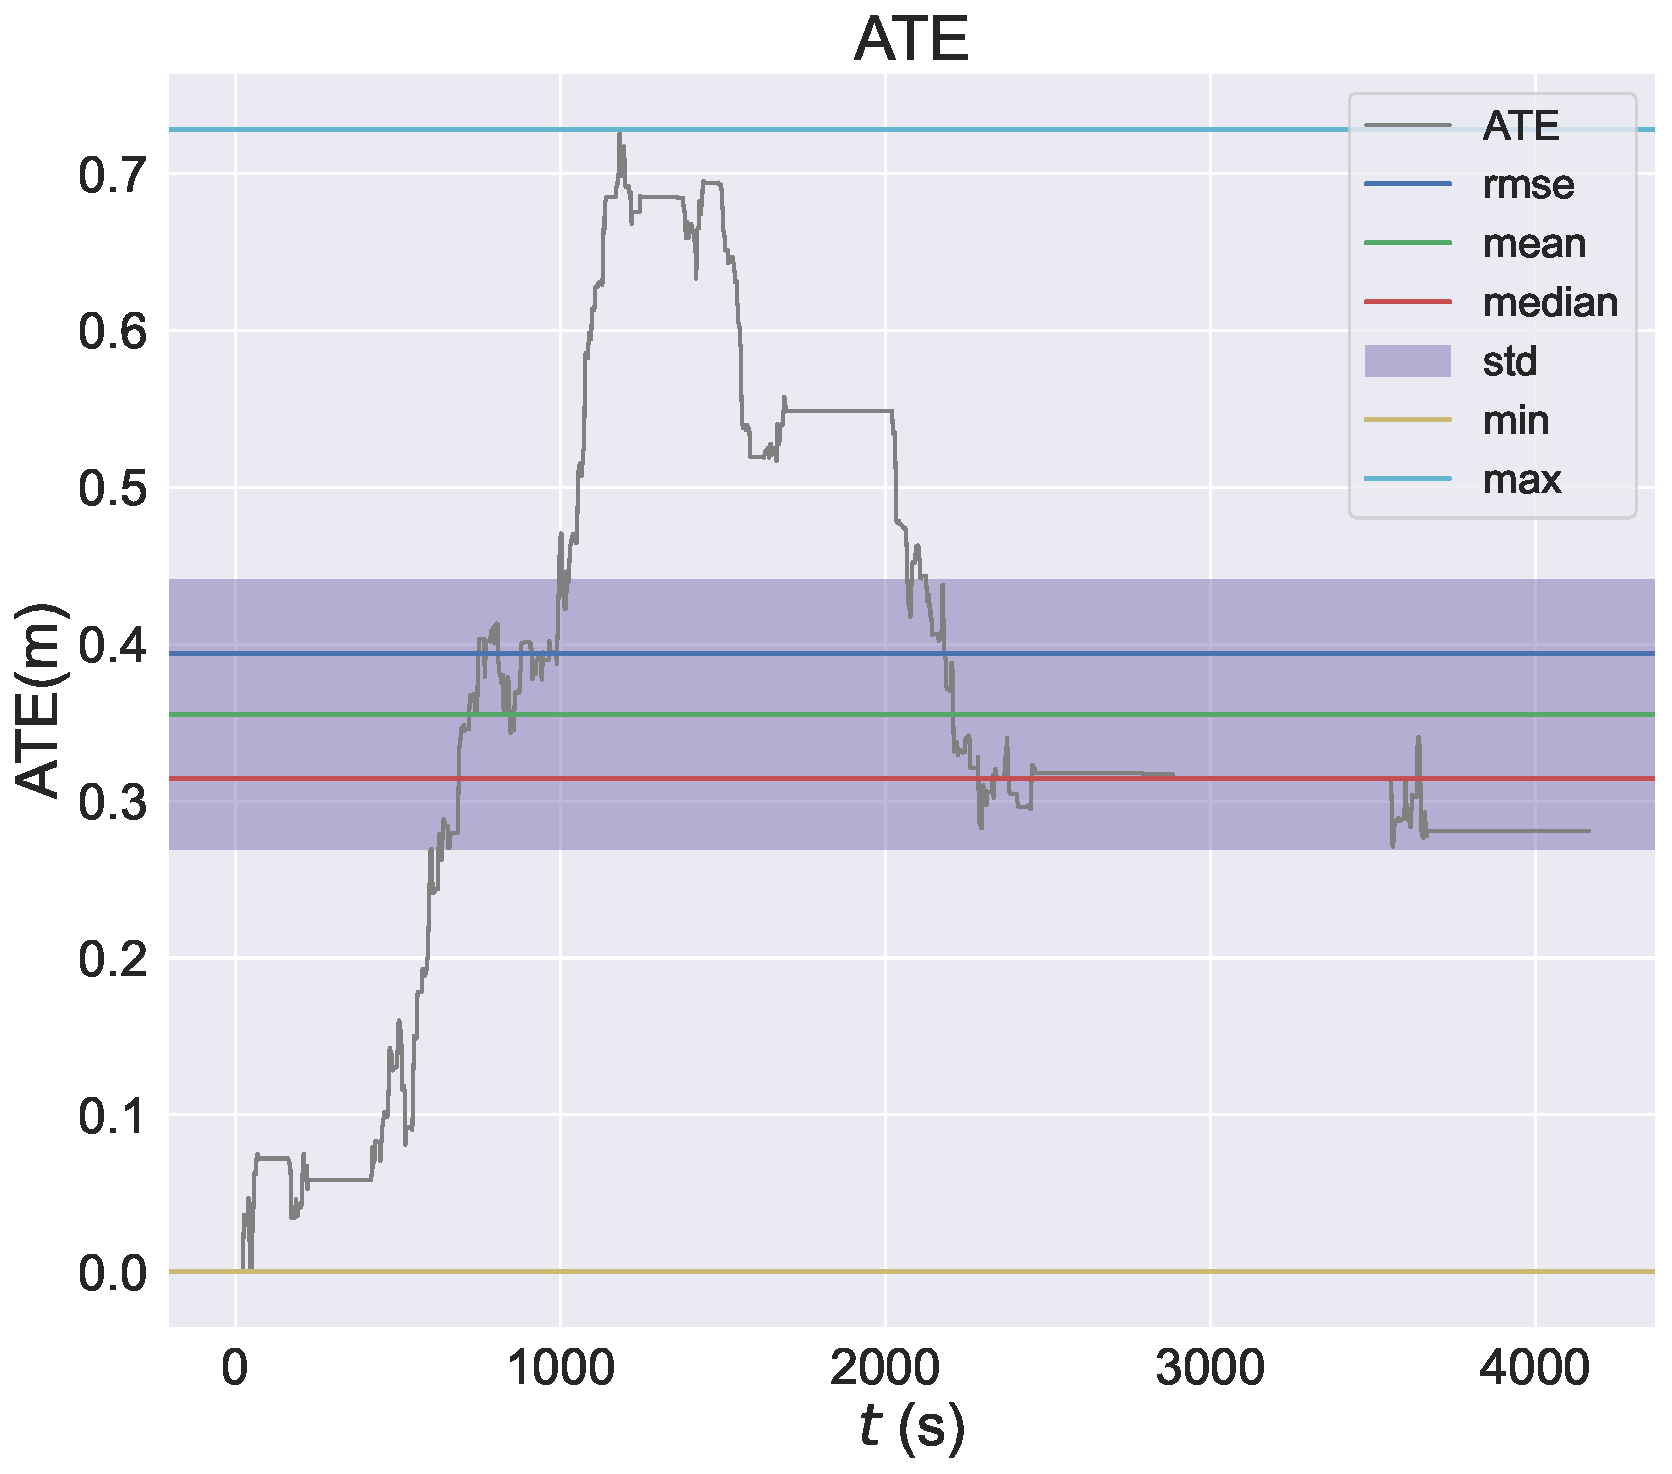
\includegraphics[width=\linewidth]{figures/APE.pdf}
        \caption{ATE variation over time}
        \label{fig:APE}
    \end{minipage}\hfill
    \begin{minipage}{0.48\textwidth}
        \centering
        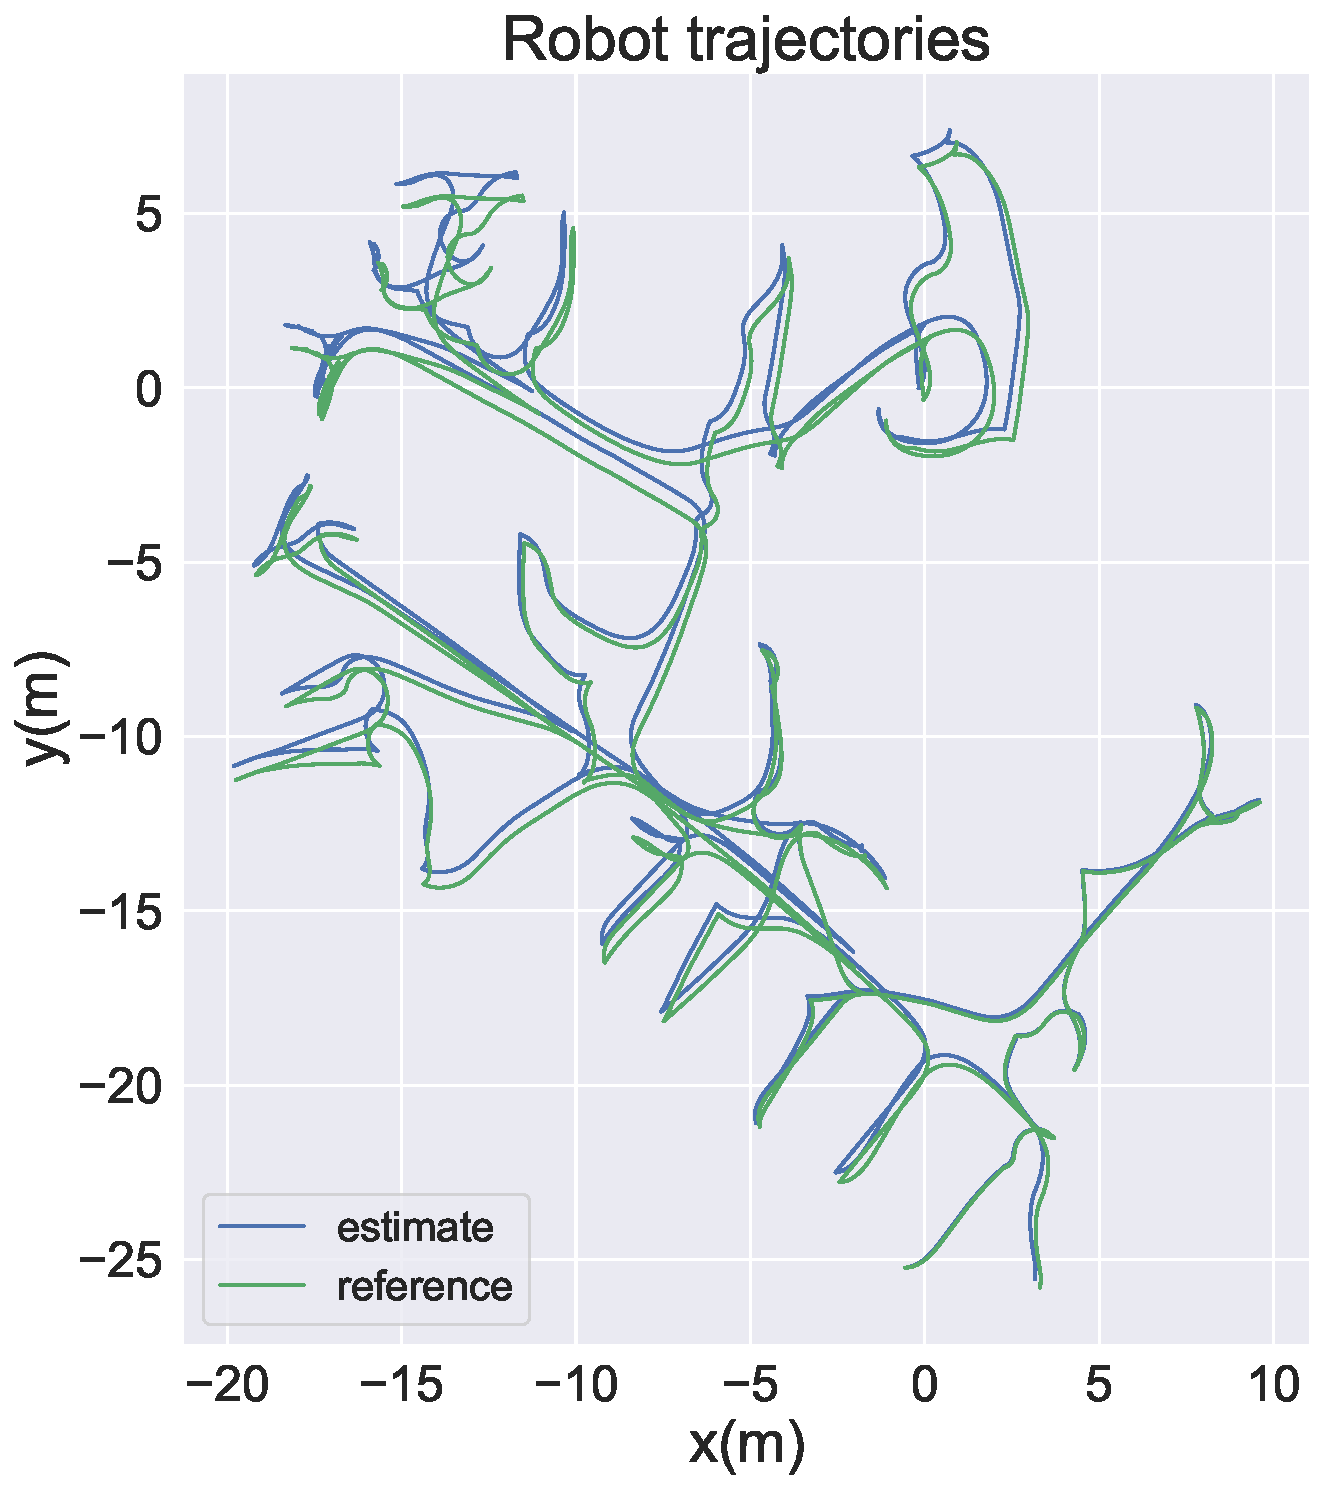
\includegraphics[width=\linewidth]{figures/trajectories.pdf}
        \caption{Difference between real (in green) and estimated (in blue) trajectory}
        \label{fig:trajectories}
    \end{minipage}
\end{figure}

\subsection{APE calculation}
As anticipated in the previous section, the APE metric is based on the difference between the estimated robot 
poses and the corresponding ground truth poses. 

Formally, let $\bm{x}_{1:T}$ be the poses of the robot estimated by
a SLAM algorithm from time step 1 to $T$, and let $\bm{x}^*_{1:T}$ be the corresponding ground truth poses.

Let $\delta_{i,j}$ be the relative transformation that moves the robot from pose $x_i$ to $x_j$:
$$ \delta_{i,j}=x_j\ominus x_i $$
$$ \delta^*_{i,j}=x^*_j\ominus x^*_i $$ 

Let $trans(\cdot)\in\mathbb{R}^2$ be the function that extracts the translational (position) component from a 
transformation, and let $rot(\cdot)\in\mathbb{R}^2$ extract the rotational (orientation) component as Euler angle.

Finally, to compute the APE: 
$$
\begin{aligned}
    \displaystyle
    \text{APE} &= \underbrace{\frac{1}{N}\sum_{i,j}trans(\delta_{i,j}\ominus\delta^*_{i,j})^2}_{\text{ATE}}+
                  \underbrace{\frac{1}{N}\sum_{i,j}rot(\delta_{i,j}\ominus\delta^*_{i,j})^2}_{\text{ARE}} \\
\end{aligned}
$$

\subsection{Project goal}
Typically, the APE is calculated a posteriori, after the robot has explored the entire environment. The main
goal of this project is to propose a predictor for the SLAM performance, specifically the APE, before running 
the algorithm or during its execution, using features derived from the input data or intermediate results.
This type of prediction can improve the robustness and efficiency of autonomous mobile systems since the 
position error (APE) can be used to correct the robot trajectory.

The work in \cite{Luperto} proposes two main APE predictors, one based on linear regression, and another one
based on a Gaussian Process via an RBF Kernel. Although Gaussian Process regression showed slightly better
performance compared to linear regression model, the authors preferred linear regression because they
considered it a more interpretable model. In both cases, a feature extractor is used \cite{Luperto2} obtaining
a set of structural features to represent the environment as a vector, which is then passed to the model.


\section{Model}
In this project, a modern Convolutional Neural Network (CNN) is used, in order to delegate the feature 
extraction to the model and directly using the environment floorplan image.
Formaly, the model $h$ we want to learn can be expressed as follows:
$$ h: [0,255]^{n,n} \times \mathbb{R}^+ \rightarrow \mathbb{R}^2 $$
Where $[0,255]^{n,n}$ is a floorplan image, encoded as a $n\times n$ grayscale image, $\mathbb{R}^+$ is the
area of the floorplan expressed in $m^2$ and $\mathbb{R}^2$ contains ATE ($m$)
and ARE ($rad$).

\subsection{Data preprocessing}

\clearpageS
\printbibliography

\end{document}